
%%%%%%%%%%%%%%%%%%%%%%% file typeinst.tex %%%%%%%%%%%%%%%%%%%%%%%%%
%
% This is the LaTeX source for the instructions to authors using
% the LaTeX document class 'llncs.cls' for contributions to
% the Lecture Notes in Computer Sciences series.
% http://www.springer.com/lncs       Springer Heidelberg 2006/05/04
%
% It may be used as a template for your own input - copy it
% to a new file with a new name and use it as the basis
% for your article.
%
% NB: the document class 'llncs' has its own and detailed documentation, see
% ftp://ftp.springer.de/data/pubftp/pub/tex/latex/llncs/latex2e/llncsdoc.pdf
%
%%%%%%%%%%%%%%%%%%%%%%%%%%%%%%%%%%%%%%%%%%%%%%%%%%%%%%%%%%%%%%%%%%%


\documentclass[runningheads,a4paper]{llncs}

\usepackage{amssymb}
\setcounter{tocdepth}{3}
\usepackage{graphicx}
\usepackage{epstopdf}
\usepackage{listings}

\usepackage{url}
\urldef{\mailsa}\path|{ales.komarek, jakub.pavlik.7, vladimir.sobeslav}@uhk.cz|    
\newcommand{\keywords}[1]{\par\addvspace\baselineskip
\noindent\keywordname\enspace\ignorespaces#1}

\begin{document}

\mainmatter  % start of an individual contribution

% first the title is needed
\title{Ontology for OpenStack Service Architectures}

% a short form should be given in case it is too long for the running head
\titlerunning{Ontology for OpenStack Service Architectures}

% the name(s) of the author(s) follow(s) next
%
% NB: Chinese authors should write their first names(s) in front of
% their surnames. This ensures that the names appear correctly in
% the running heads and the author index.
%
\author{Ales Komarek\and Jakub Pavlik\and Vladimir Sobeslav}
%
\authorrunning{Lecture Notes in Computer Science: Authors' Instructions}
% (feature abused for this document to repeat the title also on left hand pages)

% the affiliations are given next; don't give your e-mail address
% unless you accept that it will be published

\institute{Faculty of Informatics and Management, University of Hradec Kralove,\\
Rokitanskeho 62, 50003 Hradec Kralove, Czech Republic\\
\mailsa\\
\url{http://cepsos.cz}}

%
% NB: a more complex sample for affiliations and the mapping to the
% corresponding authors can be found in the file "llncs.dem"
% (search for the string "\mainmatter" where a contribution starts).
% "llncs.dem" accompanies the document class "llncs.cls".
%

\toctitle{Lecture Notes in Computer Science}
\tocauthor{Authors' Instructions}
\maketitle

\begin{abstract}
%\boldmath

This paper explains how ontology can be used to model various OpenStack architectures. OpenStack is the largest open source cloud computing IaaS platform. It has been gaining wide spread popularity among users as well as software and hardware vendors over past few years. It's a very flexible system that can support a wide range of virtualization scenarios at any scale.

In our work we propose a formalization of OpenStack architectural model that can be automatically validated and serve suitable meta-data to configuration management tools. The OWL-DL based ontology defines service components and their relations and  provides foundation for further reasoning. Provided models can support simple all-in-one architecture as as well as large architectures with service components in High Availability setup.
\keywords{OpenStack, SOA, MDA, etc.}

\end{abstract}


\section{Introduction}

%proč OpenStack - protože komunita 500000 vývojářů, tisíce firem, nárůst kódu za poslední dobu stacalytics.com 
% How OpenStack Works?

%vendor lockin, scalability from notebook to thousans of servers like CERN

% 2,292 Companies; 8,066 Individual Members; 130 Countries; 2,007 Total Contributors; 341 Average Monthly Contributors; 89,156 Code Contributors - more information at 
% www.stackalytics.com July 2014

OpenStack is the largest open-source cloud computing platform today. Many companies participate to its code, extend core functions and write new service backends to fit their business goals. The actual system consists of many components designed with plugin architecture that allows custom implementations for various service backends. These components can be combined and configured to match available software and hardware resources and real use-case needs.

Each implementation has its own component combination and use some form of configuration management tool to enforce the service states on designated servers and possibly other network components. These tools require data that covers configuration of all components. Detecting component inconsistencies by hand is painful and time consuming process.

We propose a formalization of OpenStack service architecture model, based on the approaches developed in classic knowledge representation domain, especially Service-Oriented Architecture by OpenGroup. Component definition is encoded in an ontology using the standard OWL-DL language, which enables sharing of knowledge about configurations across various systems. Reasoning can be used on the specification to automate validation of configuration changes.

When dealing with hundreds of components with thousands of properties and relations, keeping track of changes throughout its life cycle is very challenging. Current approaches are ad hoc, even OpenStack Fuel has severe limitations, there exists no standard for specifying common OpenStack architectural model. The question how to convert the proposed OWL-DL schema to metadata format that configuration management tools can process is discussed. We are working on external node classification service that uses graph database to serialize the OWL ontology with REST API that configuration management tools can use as metadata provider. This can streamline the process of adopting new services and service backends in predictable manner.

\subsection{Use Cases}

OpenStack is system that has growing number of components with growing number of components and drivers. As we will show in following text there's no universal installation of OpenStack.  

% představit OpenStack jako systém s rolemi, konfiguracemi, komponenty, drivery. jina instalace per use case. Nexexistuje univerzální instalace. Vysoka komplexita, services

\subsection{Infrastructure Modeling}

Tools usually collect required metadata through web forms or answer files. This is not a conceptual way to describe model.

% Jak vytvořit high level model (logické schéma) architektury? a přenést ji do low level design realizace? 
% Jak správně definovat architekturu na základě hw infrastruktury a target use case?

\subsection{Process Automation}

% Jak celý proces deploymentu automatizovat?



\section{Architectural Models}

Jak funguje IaaS ve smyslu deploye masiny z pohledu controlleru - zavola scheduler, ten comupte, ten pak glance, pak pripadne cinder a neutron a pusti boot, kdyz to ma ready. a tim padem provoz.

obzrazel

\subsection{Architectural Level}

OpenStack is complete Infrastructure as a Service platforms. It allows to create virtual servers on virtual networks using virtual block devices. These core services are followed by growing number of services covering for example telemetry, orchestration or data processing. All services within OpenStack architecture have pluggable backends. This allows vendors to develop plugin for their resources, that can be accessed and managed by the OpenStack API.

Figure X shows the basic configuration of OpenStack in Icehouse version.

Klasicky logicky model openstack architektury

2) OpenStack architecture moduls

Rozebrat services a představit modularitu a vendor plugins, drivers

Database

Message queue

Time service

Identity - Keystone

Image - Glance

Compute - Nova

Network - Neutron

Volume - Cinder

\subsection{Solution level}

Real implementations of Architectural models

\subsubsection{IaaS controller support}

Cluster software
- corosync/pacemaker
- keepalived

Database
- mysql/galera
- postgressql/xtradb

RPC
- rabbitmq
- qpid
- 0mq

time

\subsubsection{Iaas Controller services}

Pluggable backends

Keystone
- file
- sql
- ldap

Glance
- dir
- swift

Nova
- kvm
- qemu
- docker
- hyper-v

Neutron
- flat
- ovs-gre/vxlan
- sdns

Cinder
- lvms
- sans


Různé způsoby nasazení ukázky reálné architektury - promapovat ve 4 na ontologii

\subsection{Hardware matters}

Why we choose different openstack setups

Lab1 - 20 hypervisors, kvm, ovs-gre, local hdd
Lab2 - 4 hypervisoers, kvm, sdn-contrail, san
Lab3 - 5 hypervisors, ...



\section{OpenStack Deployment Options}

There are many ways how to deploy OpenStack infrastructure which are more or less automated. Some of them require to fill in answer files, some configuration files. Some tools have graphiceal user interface and allow to provision entire hardware infrastructure as some just configure the services on the provisioned servers.

Model je popsanej dokumentem a není to čitelný, automatizace. Není validita modelu. Chyby se debugují na úrovni reality.

\subsection{Development Environment Installers}

For testing and developing OpenStack ...

\subsubsection{PackStack}

Packstack is a utility that uses Puppet modules to deploy various parts of OpenStack on multiple pre-installed servers over SSH automatically. Currently only Fedora, Red Hat Enterprise Linux (RHEL) and compatible derivatives of both are supported.

% https://wiki.openstack.org/wiki/Packstack

\subsubsection{Devstack}

DevStack has evolved to support a large number of configuration options and alternative platforms and support services. That evolution has grown well beyond what was originally intended and the majority of configuration combinations are rarely, if ever, tested.

% http://devstack.org/overview.html

\subsection{Production Environment Managers}

For production installations of OpenStack ...

\subsubsection{Fuel}

Fuel is an open source deployment and management tool for OpenStack. Developed as an OpenStack community effort, it provides an intuitive, GUI-driven experience for deployment and management of OpenStack, related community projects and plug-ins. 

% https://wiki.openstack.org/wiki/Fuel

\subsubsection{Foreman}

You can setup Foreman to deploy RDO. The metadata is provided in Host Groups.

% https://openstack.redhat.com/Deploying_RDO_using_Foreman

\subsection{Configuration Management Tools}

You can install OpenStack by configuration management tool

\subsubsection{Puppet}

It's already used by Fuel an Foreman

\subsubsection{Salt}

Salt is another approach to install OpenStack.


\section{Ontology of OpenStack System}

\subsection{Serialization Formats}

Způsoby serialiazce ontologie

\subsubsection{XML Documents}

RDF format

\subsubsection{Graph databases}

Preserving RDF format, just very different implementation 

je to servica, tzn overhead oproti xml filu, ale zas ma api atd ...

\subsubsection{Hierarchical}

Subject (id) or property driven

\subsection{Comparison}

Srovnání jednolivých formátů pro ontologii pro openstack řešení - bezpečnost, rychlost, integrace

- speed - parsing / scaling
- integration, maintenance costs
- security issues



\section{Ontology Usage}

We chose the Opengroup's Service Oriented Architecture as a 

\subsection{Ontology details}

\begin{figure}[!h]
\centering
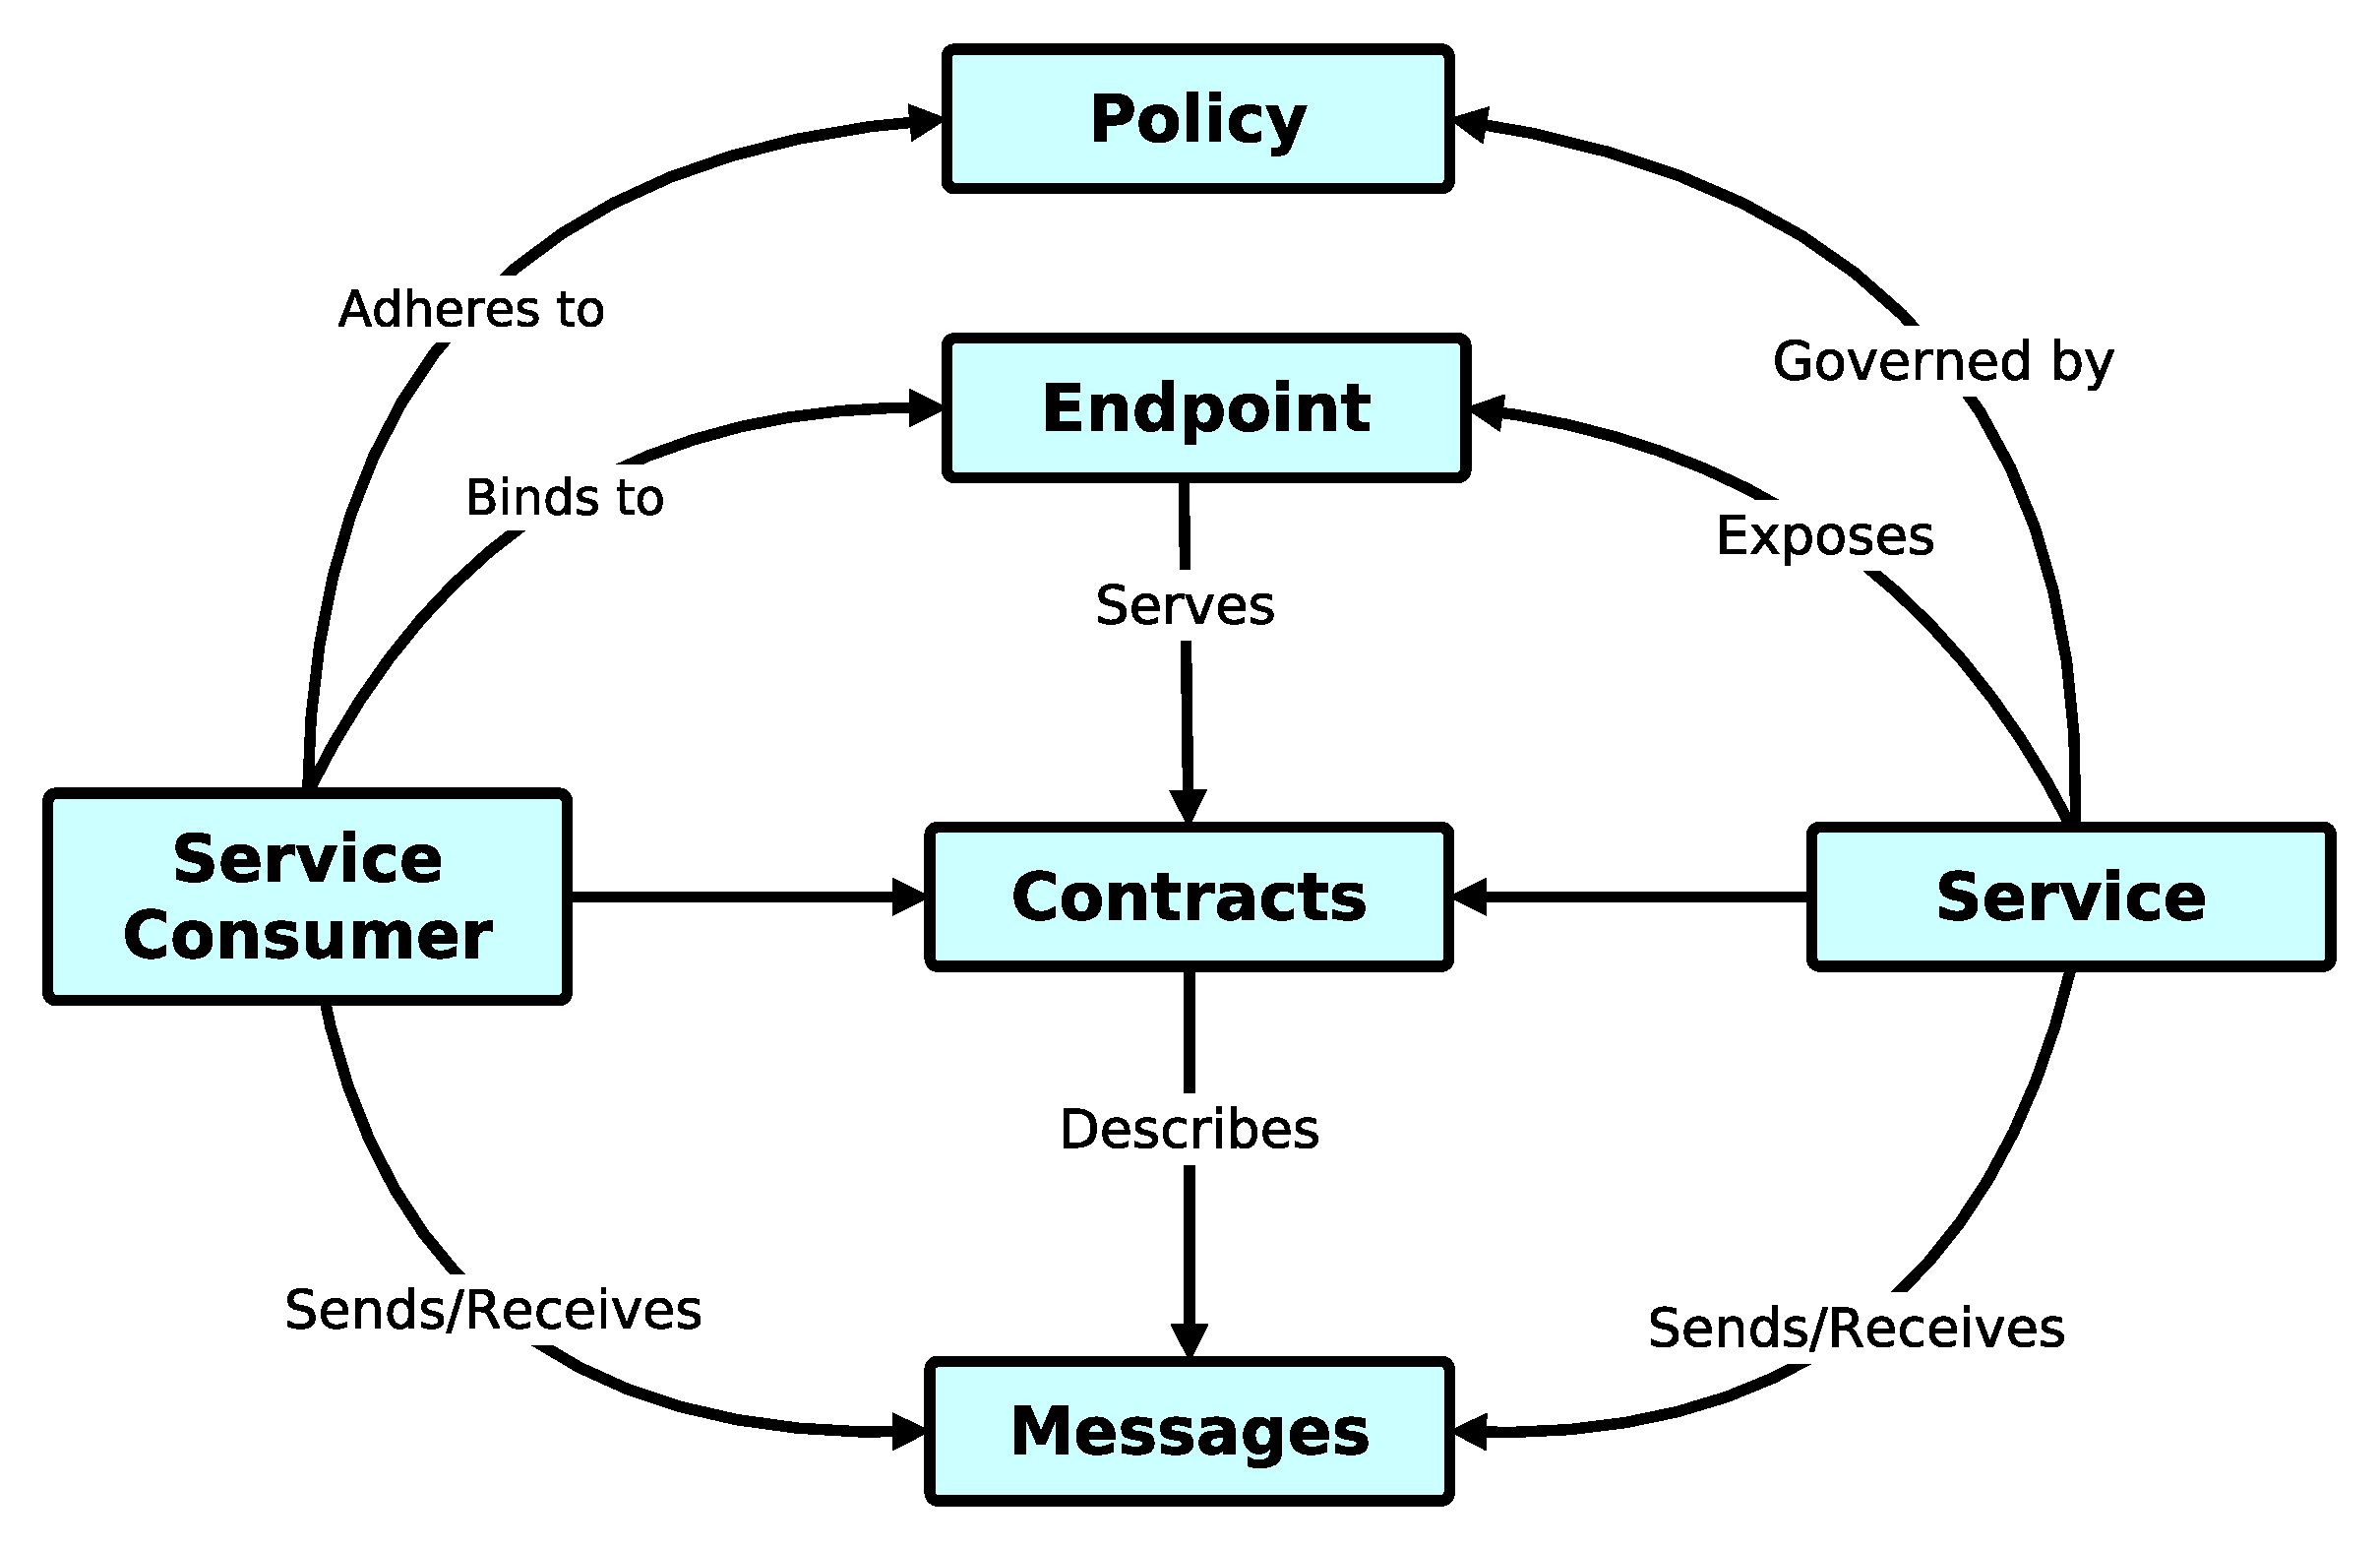
\includegraphics[scale=.2]{img/soa_relation.eps}
\caption{SOA service to consumer}
\label{fig:cm}
\end{figure}




\begin{figure}[!h]
\centering
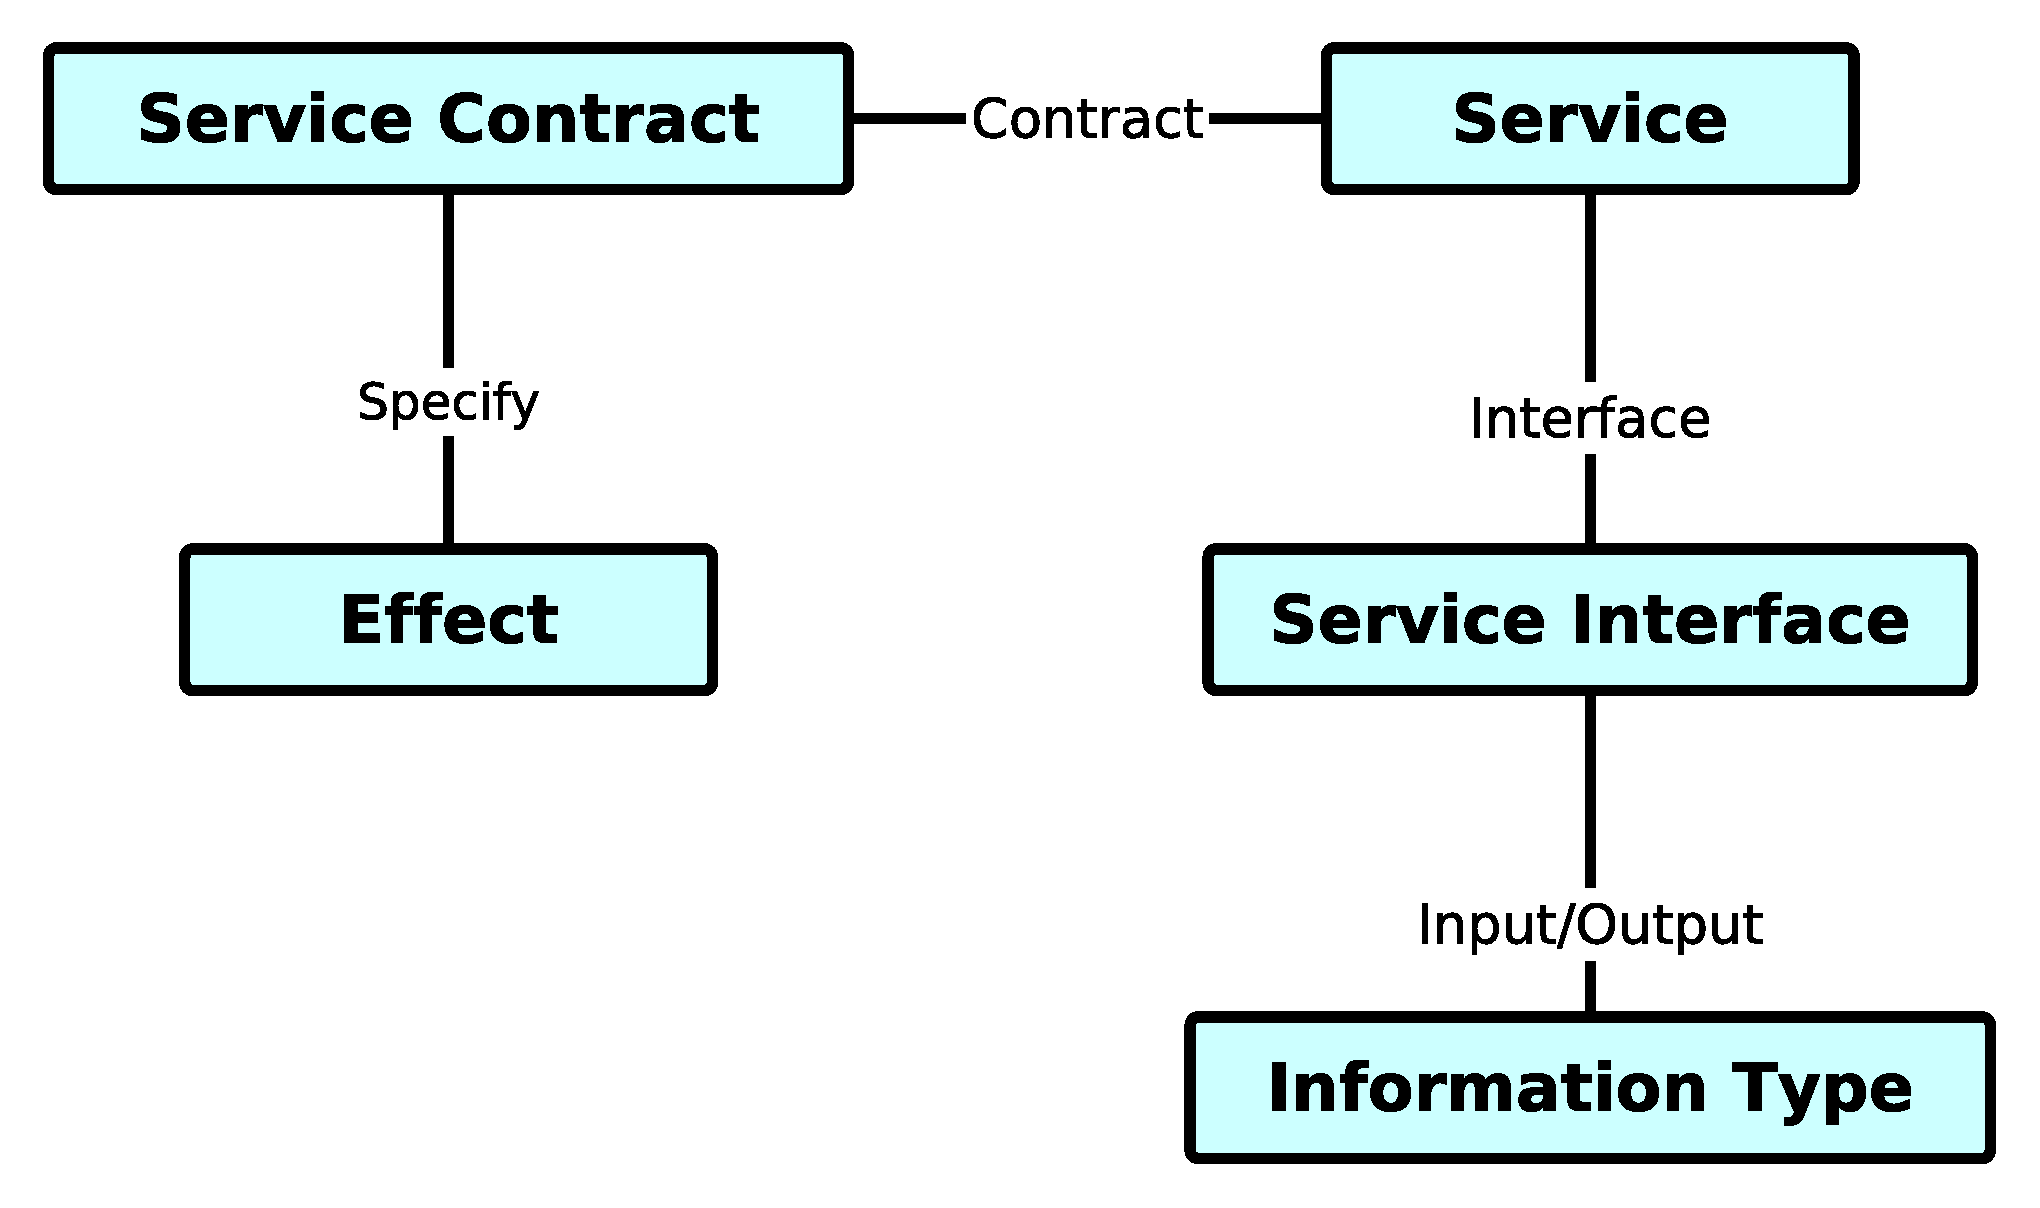
\includegraphics[scale=.2]{img/soa_property.eps}
\caption{SOA service properties}
\label{fig:cm}
\end{figure}

\subsection{Reasoning}

Deployment bez implementačních chyb.

\subsubsection{Model Integrity Validation}

Validace celého řešení vůči high level modelu.

\subsection{External Node Classification}

Mapování vybraného formátu na OpenStack

(HA architektura SDN controller)

\begin{figure}[!h]
\centering
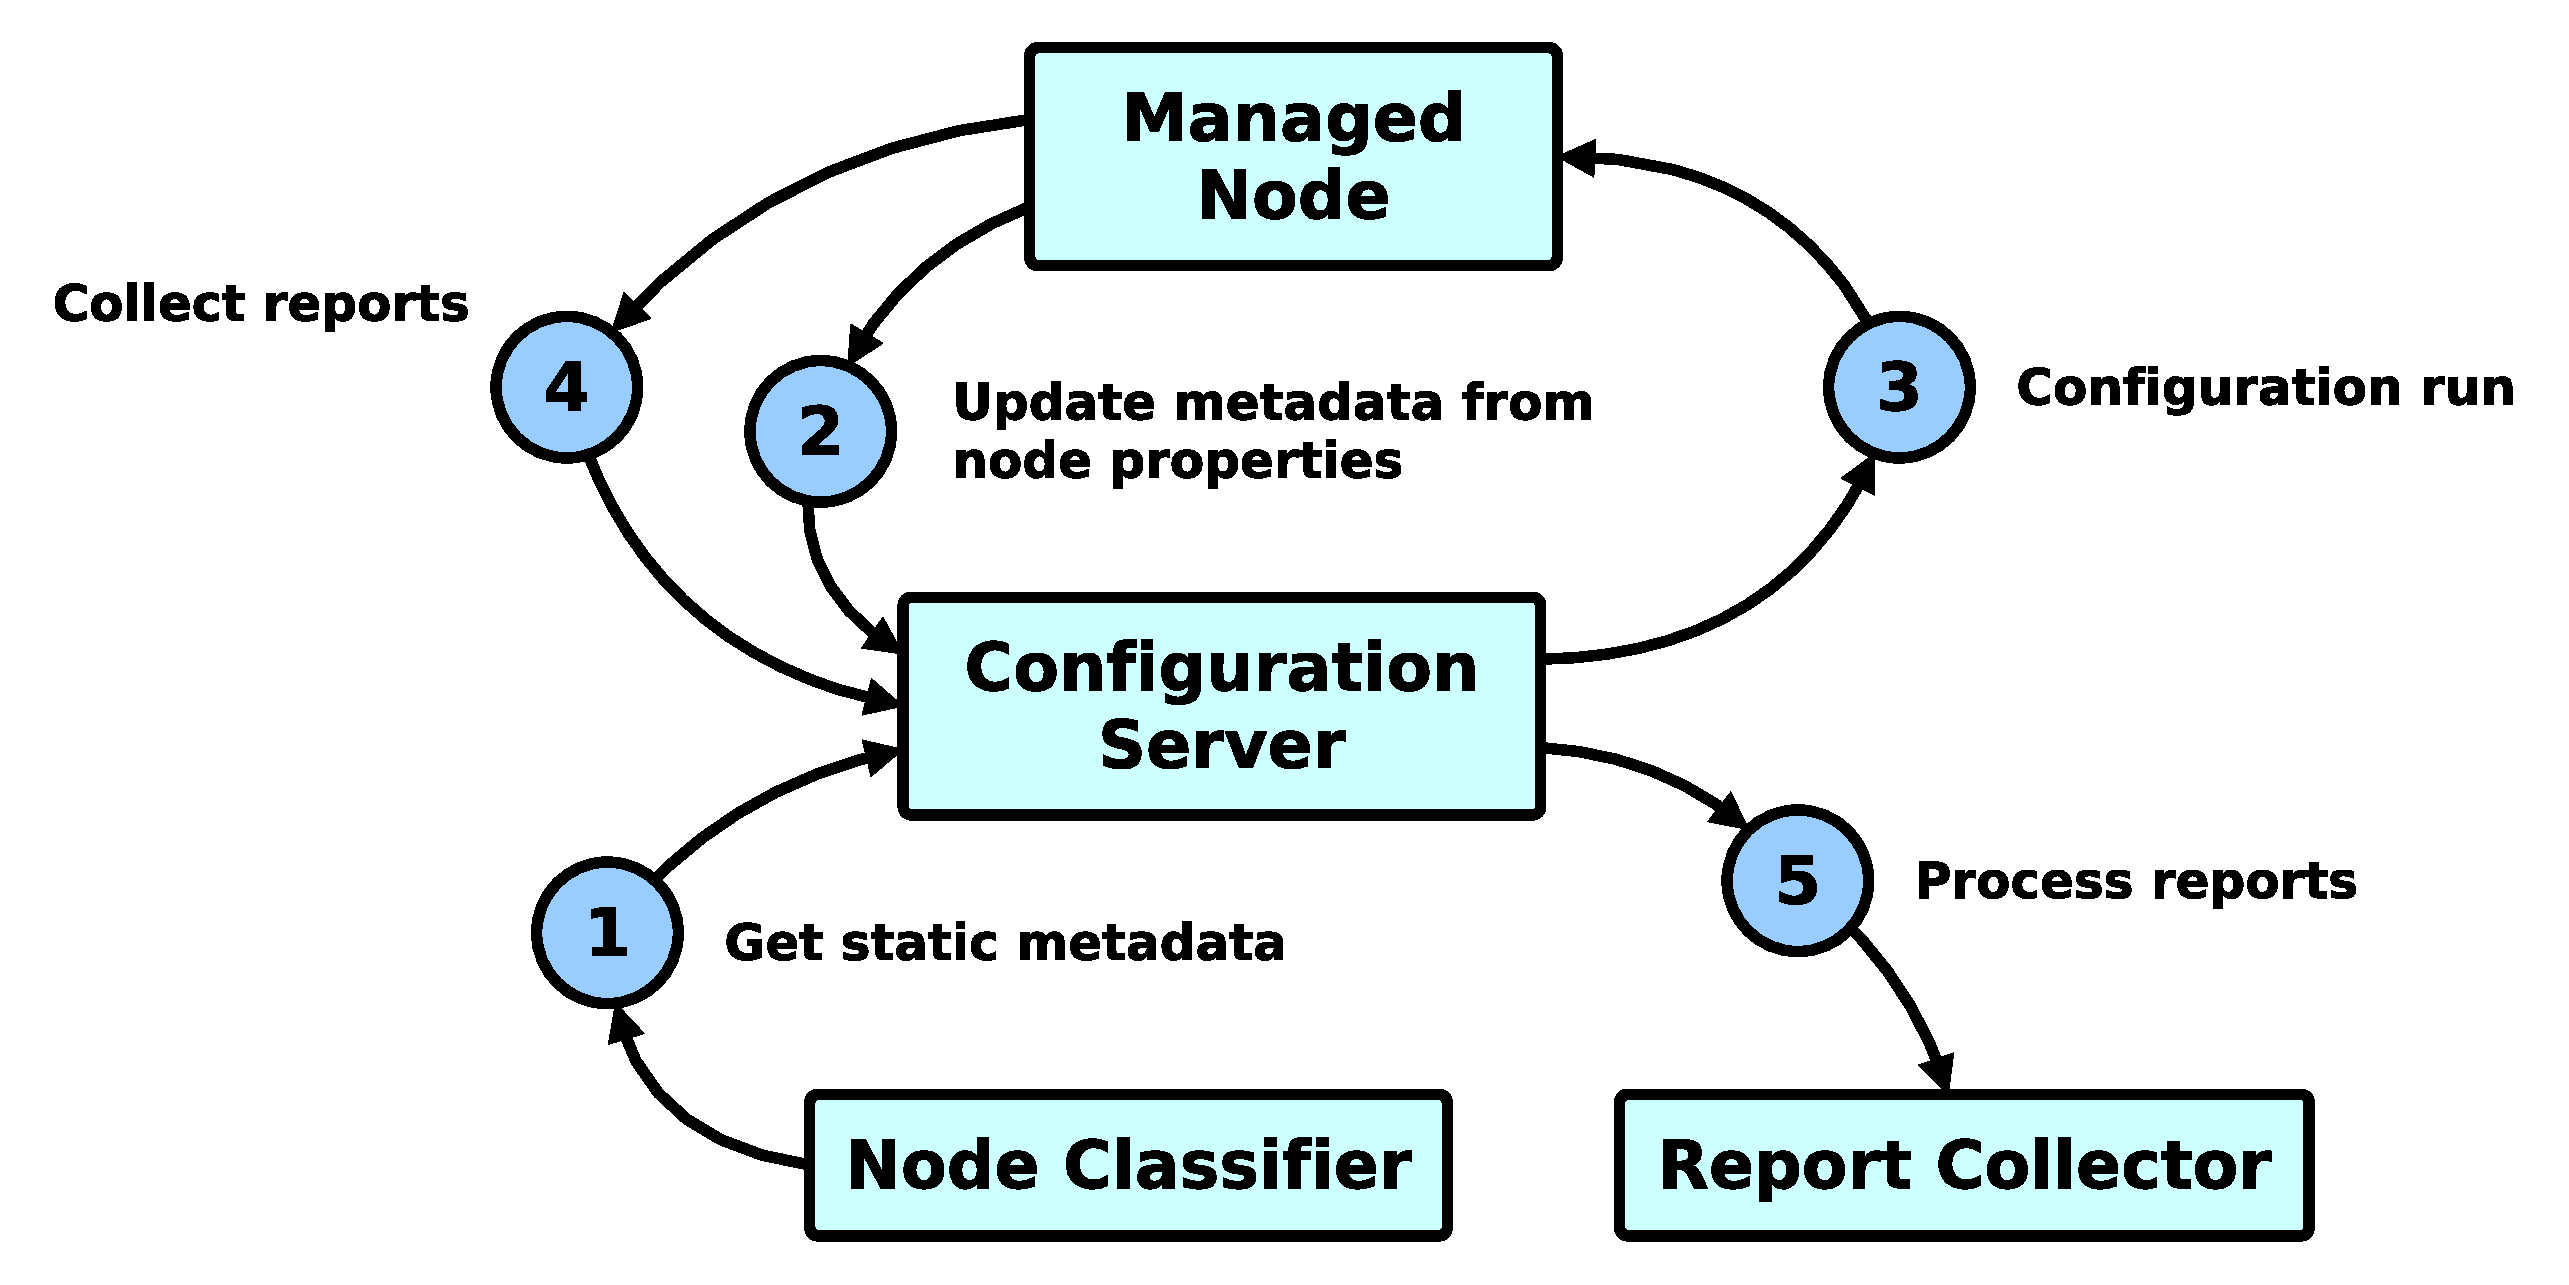
\includegraphics[scale=.15]{img/cm_cycle.eps}
\caption{Configuration Management deployment cycle}
\label{fig:cm}
\end{figure}

\subsubsection{Puppet ENC}

\subsubsection{SaltStack ENC}

Reálný přínos celého řešení


\section{Conclusion}

We have managed to do the first steps in formalization of IaaS Architecture high level models. The representation of models, the ontologies, can be used to create and validate meta-data for individual OpenStack cloud installations. The ontology provides schema for the meta-data for each installation so the overall service integrity is ensured.

We created a python-based web service django-enc that use data from the ontology to generate the suitable meta-data for configuration management tools. The service provide simple interface for manipulating the ontology as well as interfaces for ontology editors. The ontology defines the basic services of OpenStack Havana and Icehouse versions. New components and service backends can be easily defined and included.

% Ontologická reprezentace prostředí, která je vhodná pro agentové prostředí, aby bylo možné provádět autonomní rozhodnutí. 

%\subsection{Future work}

We plan to expand  ontology from virtual and physical servers to network and storage resources by better adoption of configuration management tools. Ontology model is suitable for software agent processing and their rational decisions. It is possible to define agents that will maintain the state of services according to the high-level model. The more parts of the process are modelled and their deployment automated the more manageable the whole system becomes.

\subsubsection*{Acknowledgments.}
 
The paper is supported by the project of specific science Smart networking \& cloud computing solutions (FIM, UHK, SPEV 2015).


\begin{thebibliography}{4}


% http://ryandlane.com/blog/2014/08/04/moving-away-from-puppet-saltstack-or-ansible/

% http://ryandlane.com/blog/2014/08/26/saltstack-masterless-bootstrapping/

\bibitem{NIST}
\newblock {\em  NIST. The NIST Definition of Cloud Computing}
\newblock http://csrc.nist.gov/publications/nistpubs/800-145/SP800-145.pdf

\bibitem{CloudServices}
Ivan Ivanov, Marten van Sinderen and Boris Shishkov, editors.
\newblock {\em Cloud Computing and Services Science }
\newblock Springer Science, 978-1461423256, New York, USA, 2012

\bibitem{OpenStackFuel}
\newblock {\em OpenStack. Fuel Wiki }
\newblock https://wiki.openstack.org/wiki/Fuel

\bibitem{CloudStack}
\newblock {\em CloudStack. Open Source Cloud Computing: Apache CloudStack}
\newblock http://cloudstack.apache.org/about.html

\bibitem{DevStack}
\newblock {\em Fedora Project. OpenStack devstack}
\newblock http://fedoraproject.org/wiki/OpenStack\_devstack

\bibitem{ReClass}
\newblock {\em reclass. Recursive external node classification }
\newblock http://reclass.pantsfullofunix.net/

\bibitem{Cfengine}
\newblock {\em CFEngine. FCEngine 3.5 Dcoumentation }
\newblock https://cfengine.com/docs/3.5/index.html

\bibitem{PuppetHiera}
\newblock {\em Puppet Labs. Creating Hierarchies }
\newblock http://docs.puppetlabs.com/hiera/1/hierarchy.html

\bibitem{ForemanCompute}
\newblock {\em The Foreman. The Manual: Compute Resources }
\newblock http://theforeman.org/manuals/1.4/index.html\# 5.2ComputeResources


\end{thebibliography}

\end{document}
